\documentclass[11pt]{sig-alternate}
\usepackage{tabularx}
\usepackage{graphicx}
\usepackage{blindtext}
\usepackage[utf8]{inputenc}
\usepackage[english]{babel}
\usepackage{lastpage}
\usepackage{comment}
\usepackage{dirtytalk}
\usepackage{xcolor}
\usepackage{hanging}
\usepackage{wrapfig}
\usepackage[backend=biber, style=apa]{biblatex}
\addbibresource{notation.bib}
\usepackage{authblk}
\usepackage{caption}
\usepackage{subcaption}
\usepackage{graphicx,subfigure}
\usepackage{authblk}
\usepackage{enumitem}
\usepackage[utf8]{inputenc}
\usepackage{cuted}
\usepackage{fancyhdr}
\usepackage{xurl}
\usepackage{multirow}
\usepackage{hyperref}
\pagestyle{fancy}
\renewcommand{\headrulewidth}{0pt}
\renewcommand{\footrulewidth}{0pt}
\setlength\headheight{80.0pt}
\addtolength{\textheight}{-80.0pt}
\chead{%
  \ifcase\value{page}
  % empty test for page = 0
  \or 
\includegraphics[width=\textwidth]{headerImage.png}% page=1
  \or 
\includegraphics[width=\textwidth]{headerImage.png}% page = 2
  \or 
\includegraphics[width=\textwidth]{headerImage.png}% page = 3
  \or 
\includegraphics[width=\textwidth]{headerImage.png}% page = 4
  \or 
\includegraphics[width=\textwidth]{headerImage.png}% page = 5
  \else
  
\includegraphics[width=\textwidth]{headerImage.png}
  \fi
}
%\chead{
\includegraphics[width=\textwidth]{headerImage.png}}
\fancyfoot[LE,LO]{Making Environmental Education Accessible for All Students: Inclusion of Students with Emotional and Behavioral Disabilities\\           
DOI: 10.14448/jsesd.13.0004}
\fancyfoot[CE,CO]{{ }}
\fancyfoot[RE,RO]{\thepage}
\pagenumbering{arabic}
\hypersetup{
    colorlinks=true,
    urlcolor=blue
}
 
\let\oldabstract\abstract
\let\oldendabstract\endabstract
\makeatletter
\renewenvironment{abstract}
{\renewenvironment{quotation}%
               {\list{}{\addtolength{\leftmargin}{1em} % change this value to add or remove length to the the default
                        \listparindent 1.5em%
                        \itemindent    \listparindent%
                        \rightmargin   \leftmargin%
                        \parsep        \z@ \@plus\p@}%
                \item\relax}%
               {\endlist}%
\oldabstract}
{\oldendabstract}
\makeatother

% Left align captions
\captionsetup{justification   = raggedright,
              singlelinecheck = false}
              
\begin{document}


\title{Making Environmental Education Accessible for All Students: Inclusion of Students with Emotional and Behavioral Disabilities}

\author[1]{\large \color{blue} Juliann Dupuis}
\author[2]{\large \color{blue} Dawn Jacobs}


\affil[1]{Notre Dame of Maryland University}
\affil[2]{University of Maryland College Park}

\toappear{}

\maketitle
\begin{@twocolumnfalse} 

\begin{abstract}
\begin{large}
\item 
     \textit{One of the most difficult tasks of an educator is engaging students in rigorous learning opportunities. A greater challenge is finding ways in which environmental education can be accessible to all students, especially those with Emotional and Behavior Disorders.  This article and lesson provides best practices for engaging students with Emotional and Behavioral Disabilities in environmental concepts through varied representations and expressions of content. In addition, teaching collaborative protocols to fully engage students with social skills challenges within the local environment are discussed. The instructional approaches are aligned to increasing academic discourse, building positive peer-peer relationships, and observation using multiple modalities.}
     \\
     \\
    \textbf{Keywords:} science, students with disabilities, practitioners, instruction, strategies, supports, teaching, techniques
\end{large}
\end{abstract}
\end{@twocolumnfalse}

%% ABSTRACT


%% AUTHOR INFORMATION
\textbf{*Corresponding Author, Juliann Dupuis} \href{mailto:jdupuis@ndm.edu}{(jdupuis@ndm.edu)} \\
\textit{Submitted November 15, 2020}\\
\textit{Accepted January 14, 2021} \\
\textit{Published online March 28, 2021} \\
\textit{DOI: 10.14448/jsesd.13.0004} \\


\pagebreak
\pagebreak

\vspace{5mm}
\section*{\vspace{140mm}}
\begin{large}

% Please add the following required packages to your document preamble:
% \usepackage{graphicx}
\begin{table*}[h!]
\resizebox{\textwidth}{!}{%
\begin{tabular}{|l|l|}
\hline
\textbf{Content Area:} &
  Environmental Education \\ \hline
\textbf{Big Idea:} &
  \begin{tabular}[c]{@{}l@{}}Using collaborative strategies to engage in scientific exploration of ecosystems \\ within the outdoor environment.\end{tabular} \\ \hline
\textbf{Objectives:} &
  \begin{tabular}[c]{@{}l@{}}Students will be able to illustrate and describe the movement of energy between \\ organisms in a food chain/food web.\\ Students will be able to formulate and defend their rationale for the importance \\ of organisms in an ecosystem.\\ Using guidance from the partner protocol, students will engage in collaborative \\ discussions to record shared scientific observations during outdoor exploration.\\ Students will support one another during outdoor exploration by utilizing problem-\\ solving norms and complimenting partner contributions.\end{tabular} \\ \hline
\textbf{Time Needed:} &
  \begin{tabular}[c]{@{}l@{}}Two 40–50-minute class periods (Engage, Explore).\\ One 60-minute class period (Explain, Elaborate, and Evaluate)\end{tabular} \\ \hline
\end{tabular}%
}
\end{table*}

\section*{Introduction}
Environmental education is important for students to experience firsthand in order to make a lasting impression and provide authentic experiences. Science educators are responsible for engaging students in rigorous outdoor learning opportunities, which can become daunting when identifying ways to make environmental education accessible to all students, including those navigating behavior challenges. Students with classified Emotional and Behavior Disorders (EBD) may display behaviors such as aggression towards instructors and peers (i.e., verbal and physical threats), opposition to directions, and even elopement from the classroom. Given the severity of the behaviors, the tendency of many teachers is to avoid activities in new outdoor settings and eliminate cooperative learning opportunities. These practices occur despite evidence that science education is highly effective when applied outdoors. In addition, cooperative learning practices increase empathy and reduce bullying in middle school settings (Kendrick et al., 2012; Ryzin \& Roseth, 2019). Cooperative learning opportunities can help to build social support networks, which are cited as a buffer or preventative factor against two negative outcomes, stress (Cassell, 1974; Cutrona \& Russell, 1990; House, 1981; Lin \& Ensel, 1989) and depression (Alloway \& Bebbington, 1987; Fiore et al., 1986), because they help the recipient cope when difficult life events occur.

Furthermore, according to the National Assessment of Educational Progress (NAEP; National Center for Education Statistics [NCES], 2012) data students with disabilities perform significantly lower than their general education peers. Of children with disabilities, individuals with Emotional and Behavior Disorders have the lowest graduation rate and are three times more likely to be arrested (Data Resource Center for Child \& Adolescent Health, 2005/2006). Given these significant concerns, social support is key to intervention protocols that assist children with emotional challenges. In special education settings, there are numerous daily interaction opportunities between teachers and peers. Investigations that explore specific ways peers, instructors, and students with EBD can bolster social relationships within the classroom environment will enhance the current literature. 

In response to alarming academic trends among children with behavioral challenges, the authors of this article provide connections to current practices related to enhanced science education and social interaction. To highlight the approach, an example of a lesson that includes a peer assisted learning protocol is detailed to encourage collaborative exploration. This peer-based strategy is embedded within a 5E lesson plan format to allow for optimal student directed engagement with the content. These strategies are tied closely to literature that suggests peer-assisted support enhances access for students with disabilities (Fuchs, Fuchs, \& Burish 2000). 

The intervention protocol included in this study serves as the independent variable and student collaborative outcomes are the dependent variable. The following topics are detailed, (a) transitioning students with Emotional and Behavior Disabilities outside to conduct hands-on inquiry-based activities, (b) teaching strategies aligned to increasing academic discourse, (c) building positive peer-peer relationships, (d) and observation using multiple modalities.

\section*{Lesson Plans and Intervention}
\subsection*{Using Cooperative Learning Intervention \\Strategies in the Classroom}

The lesson described will address the academic and social needs of learners with Emotional and Behavior Disabilities during science exploration lessons. Specifically, we will include evidence-based Peer Assisted Learning Strategies (PALS) adapted from a special education peer-tutoring program to actively engage students in less structured outdoor settings (U.S. Department of Education, Institute of Education Sciences, What Works Clearinghouse, 2012, June). Typically, the PALS program is implemented as a supplemental intervention for children in elementary and middle school across reading and/or mathematics. The investigators selected an adapted version of PALS for the lessons given the benefits of cooperative learning approaches among students with Emotional and Behavioral Disabilities. The use of cooperative learning strategies in varied subjects and settings can enhance student success based upon the subsequent meaningful conversations, social supports and friendships (Kendrick et al., 2012). In addition, providing a clear protocol for collaboration bolsters academic outcomes and makes learning more accessible, especially for those that struggle with social interactions. 

Given the strong evidence surrounding peer-based intervention, it is a promising tool to incorporate in inquiry driven science lessons (Fuchs, Fuchs, \& Burish 2000; Kendrick et al., 2012). Many science teachers feel overwhelmed by the idea of taking students with Emotional and Behavioral Disabilities outside to engage in science lessons. By initiating a peer driven intervention protocol, instructors are more likely to meet specific behavioral and academic needs during outdoor learning time. The article provides targeted strategies to involve students with behavioral challenges in outdoor learning within a 5e lesson, (a) Engage, (b) Explore, (c) Explain, (d) Elaborate, and (e) Evaluate. 

\subsection*{Engage: Matching Partners }

This section should take one 20-25-minute class period. To begin the lesson sequence, utilize the Peer Assisted Learning Strategies (PALS) approach to appropriately match students (Fuchs, Fuchs, \& Burish 2000). The PALS approach allows teachers to match academically diverse students, while also considering specific instructional needs. Often, teachers simply pair students based upon ability, which prevents full access and engagement in the lesson. Instead, before the first lesson, assign partner pairs who are not too far apart academically to ensure that needs are varied within the group, the level of discussion is enhanced, and frustration is minimal. First, rank students by ability (Most Advanced= Student 1 and Lowest Scores= Student 6) and then pair them comparably (e.g., student 2 and student 5). Of course, we recognize that teachers must take personality, interest, and related needs into consideration, which may result in slightly adjusted pairs.

\subsection*{Engage: Pre-Intervention Activity}

This section should take one 20-25-minute class period. There are two components to the pre-intervention activity, an academic science focus and social-emotional collaboration observation. For the lesson one science activity, provide students with a collaborative task to complete, without any specific expectations relating to teamwork. An example of this task would be to use pictures of different organisms that would fit within each category (mammal, fish, amphibian, reptile, bird, insect) but are different enough from one another to generate discussion regarding the resulting pairs and matching rational (i.e. a cardinal and penguin). The pictures should be displayed around the room for students to visually examine and conduct observations as they try to determine the pairing. Students should note the different adaptations and/or characteristics of the organisms and how they are suited for a specific environment (Birds-wings, beaks, feathers, lay eggs). This should help them to correctly identify the organism that would be in the same category as the one they were provided. After students locate the match, they should share their rationale with the class. Specifically, why they determined their organism would be in the same category as the selected image.

Furthermore, in order for the teacher to assess changes in student collaborative behavior a pre-intervention strategy is outlined. The initial pre-intervention activities provide teachers with insight about social and collaboration needs in connection to successfully accomplishing the Next Generation Science Standards. As students engage in the science activities, the teacher should complete an observation checklist to identify student behaviors observed throughout the class. The checklist (Table 1) highlights collaborative discussion, shared responsibility for completing tasks, and positive reinforcement to one another (compliments). Students can receive up to 12 points for the observed partner engagement behaviors. Although students can demonstrate the behaviors in each category multiple times, the rating is based upon at least one observation per partner. Proficiency is rated as follows: 10-12 points (Meets Expectations), 6-9 points (Approaching Expectations), and 5 or less points (Below: Requires Intervention). The subsequent data on the observed and absent behaviors support the next steps within the planning and intervention implementation.

\begin{table*}[]
\captionsetup{font=large, labelfont=bf}
\caption{\textbf{Observation Checklist}}
\label{tab:table-1}
\resizebox{13cm}{!}{%
\begin{tabular}{|l|l|l|l|}
\hline
\multicolumn{1}{|c|}{\textbf{Observation}} &
  \multicolumn{1}{c|}{\textbf{Observed}} &
  \multicolumn{1}{c|}{\textbf{\begin{tabular}[c]{@{}c@{}}Not \\ Observed\end{tabular}}} &
  \multicolumn{1}{c|}{\textbf{\begin{tabular}[c]{@{}c@{}}Notes \\ (Optional)\end{tabular}}} \\ \hline
\begin{tabular}[c]{@{}l@{}}Both Partners add ideas (e.g. \\ Notes/Illustration) to the \\ Exploration Sheet.\\ (Danielson 3c)\end{tabular} &
   &
   &
   \\ \hline
\begin{tabular}[c]{@{}l@{}}Each partner asks a question \\ prior to exploring and/or while \\ completing the Exploration \\ Record Sheet.\\ (Danielson 3b)\end{tabular} &
   &
   &
   \\ \hline
\begin{tabular}[c]{@{}l@{}}The pair discusses answers \\ to their questions prior to \\ exploring and/or while \\ completing the Exploration \\ Record Sheet.\\ (Danielson 3b)\end{tabular} &
   &
   &
   \\ \hline
\begin{tabular}[c]{@{}l@{}}Both partners give compliments \\ to one another while exploring \\ and/or after completing the \\ Exploration Record Sheet.\\ (Danielson 2a)\end{tabular} &
   &
   &
   \\ \hline
\begin{tabular}[c]{@{}l@{}}When questioned by the teacher, \\ each partner can explain ideas \\ recorded on the Exploration \\ Record Sheet.\\ (Danielson 2d)\end{tabular} &
   &
   &
   \\ \hline
\begin{tabular}[c]{@{}l@{}}When asked to evaluate how \\ well they collaborated using a \\ scale of (1) Very Well, (2) Well, \\ (3) Just Okay, or (4) Not At All, \\ each student respond with “Well” \\ or “Very Well.”\\ (Danielson 3d)\end{tabular} &
   &
   &
   \\ \hline
\end{tabular}%
}
\subcaptionsetup{font=large}
\subcaption*{\textit{Observation checklist to be completed by teacher during engage activity and explore}}
\end{table*}

\subsection*{Explore: Intervention}

This section should take a 40-50-minute class period. In the second lesson, the teacher provides guidance to students by creating a \textit{Collaboration Compliments List}, which includes positive language for participants to utilize throughout the activity. The teacher should prompt the students to generate ideas of positive words that can be stated to encourage one another. For example, \textit{that was a great idea, do you agree or have another idea?}, etc… (See Figure 1). The teacher records these on the board on a sheet of chart paper that can be displayed in the classroom. 

\begin{figure}[h!]
    \centering
    \captionsetup{font=large}
    \caption*{\textbf{Figure 1:} \textit{Classroom example of Collaborative Compliments List}}
    \label{Figure 2}
    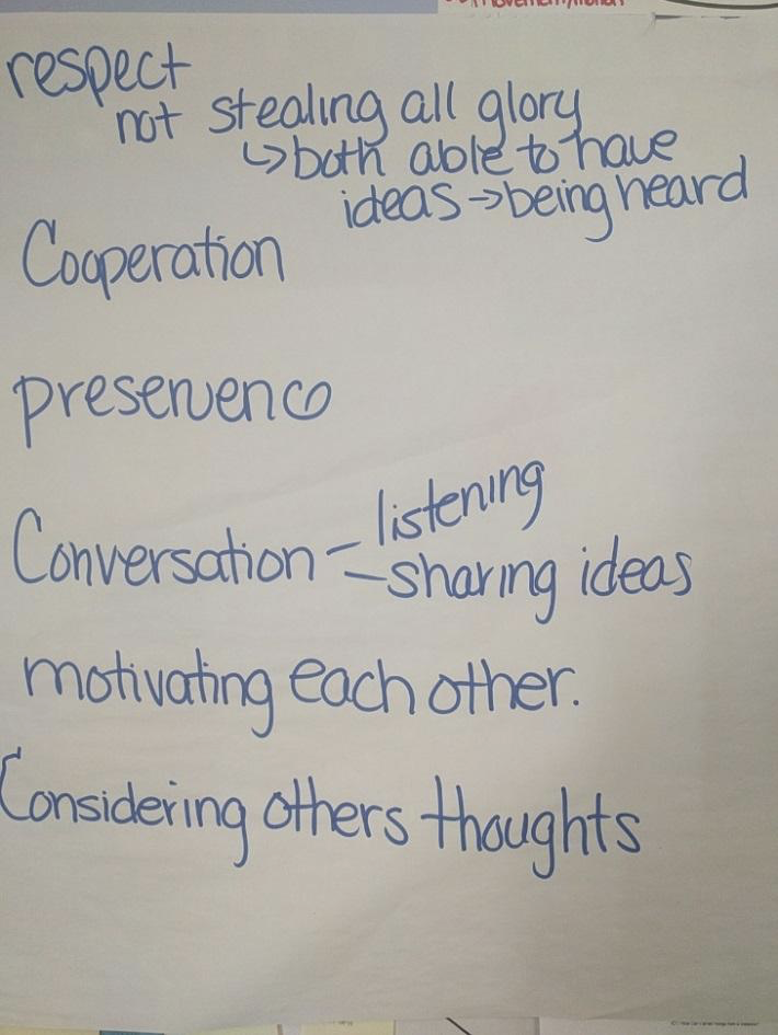
\includegraphics[width=\columnwidth]{Figure 1a.png}
\end{figure}

\newpage
\subsubsection*{Ideas for teachers to guide students while creating the collaborative compliments list}
\textbf{Collaborative Compliments List}
\begin{itemize}
    \item communication: talk to each other using inside voices and respectfully
    \item ask for clarification, what do you mean?
    \item listening: without interrupting
    \item eye contact: while the partner is speaking
    \item share your ideas: make connections
    \item ask your partner's opinion, do you agree or have another idea
    \item respect: don't steal all the glory
    \item all ideas need to be heard-considering other's thoughts
    \item cooperation, let's both talk and explore this [blank] together
    \item perseverance, you asked lots of questions to figure out the answer
    \item motivating one another, that was a great idea
\end{itemize}

Upon completion of the \textit{Collaboration Compliments List}, a partner protocol should be discussed to illustrate the dynamics of a positive learning experience with team members. In addition, the teacher should highlight questions for students to ask one another in times of disagreement. Such as, (a) why do you think we should write instead of ? (b) How can we add more detail to the drawing or answer? (c) I don’t understand your idea can you say it in a different way? (d) I disagree because. Given that the observation sheet for phrases and illustrations is shared, teachers should focus on ways to discuss differences of opinion in relation to the environmental observations. The final step in the intervention is a partner activity to enable students to practice the agreed upon compliment protocols during the outdoor activity (see Figure 2). Before going outside, students should work in their groups to complete the first Exploration Record Sheet (Figure 3) which asks students to brainstorm what they think they might see outside based on prior knowledge. While working outside students complete the second Exploration Record Sheet (Figure 3) that allows them to add observation notes of what they are actually observing, using phrases and illustrations. During the outdoor activity, the teacher should complete another observation checklist to compare observed collaborative behaviors pre and post intervention.

Before going outside, the teacher should remind students of acceptable and safe practices when engaging in outdoor experiences. Some general rules should be addressed including: Walking, staying within the boundaries provided by the teacher, leave nature in nature (no damaging of living organisms), maintain a low voice so as not to scare any potential organisms. 

\begin{figure}[h!]
    \centering
    \captionsetup{font=large}
    \caption*{\textbf{Figure 2:}\textit{ Partner protocol and norms created by students}}
    \label{Figure 2}
    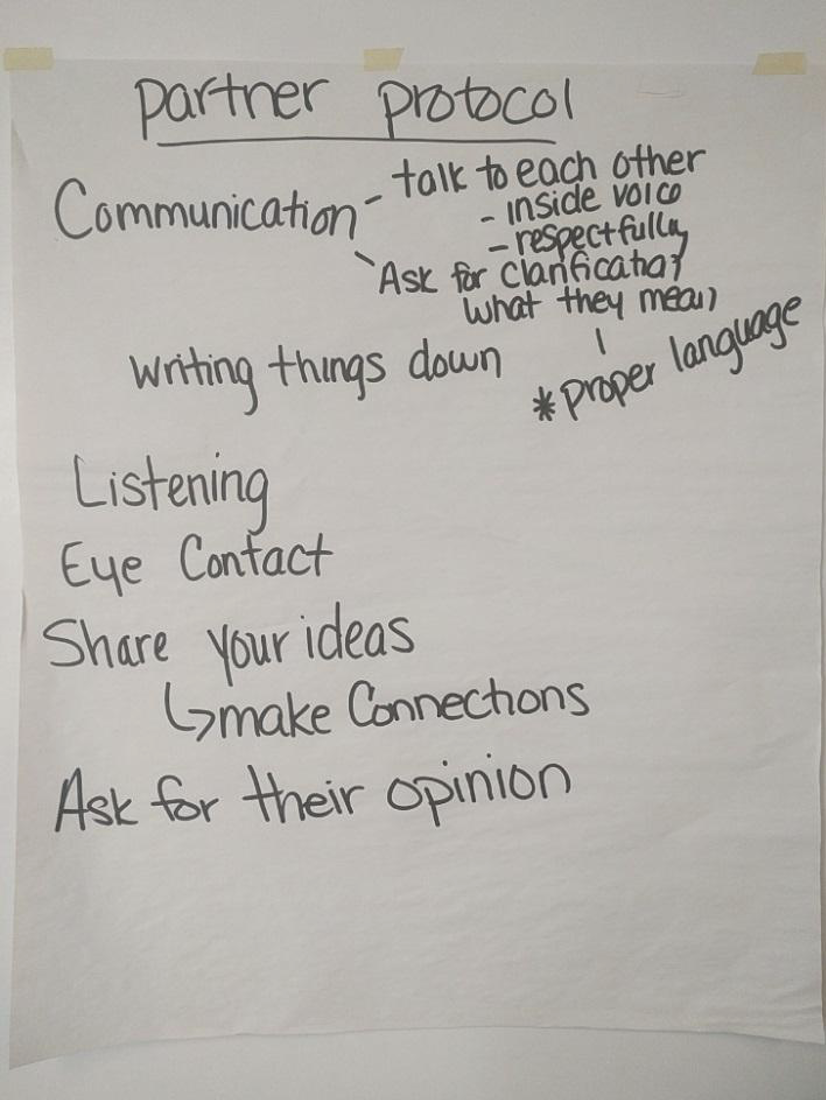
\includegraphics[width=\columnwidth]{Figure 2a.png}
\end{figure}

\subsubsection*{Partner protocol that students discuss and practice}
\begin{enumerate}
    \item Partners take turns reading the items on the "Exploration Record Sheet" (One person reads odd numbers, one person reads even numbers) out loud.
    \item Each partner asks a question about the item BEFORE looking around
    \begin{itemize}
        \item Where should we start looking?
        \item What types of things should we look for?
        \item I wonder if [blank]?
    \end{itemize}
    \item Partners discuss answers to the questions and agree where to begin exploration
    \begin{itemize}
        \item I think [blank] because [blank].
        \item I agree because [blank].
    \end{itemize}
    \item AFTER ILLUSTRATING and SCRIBING, each student provides a compliment from the list generated earlier during the introduction of the lesson.
\end{enumerate}

\subsubsection*{\textbf{Figure 3:} Exploration Record Sheet (inside)}
I spy...\\
Today you will be working in teams to explore the outdoor environment and track down examples of different types of organisms. These organisms will help to illustrate the different energy roles in an environment. But before we start our exploration there are a few important terms we need to know.

\begin{itemize}
    \item \textbf{Producer:} An organism that can make its own food. Producers are the source of all food in an ecosystem. Example-plant.
    \item \textbf{Consumer:} An organism that cannot make its own food. Feeds on other organisms. There are three types of consumers:
    \begin{itemize}
        \item \textbf{Herbivores:} Eat only plants. Example-caterpillar
        \item \textbf{Carnivores:} Eat only other animals. Example- bald eagle
        \item \textbf{Omnivores:} Eat both plants and animals. Example-squirrel
    \end{itemize}
    \item \textbf{Decomposer:} Organisms that break down wastes and dead organisms and return the raw materials to the ecosystem. Example-mushroom
\end{itemize}

\textbf{Task: Before going outside:} work with your partner to provide examples of each of the following categories of organisms that you think you will see outside during your observations. Use prior knowledge of the local ecosystem to help you brainstorm.

\begin{table}[h!]
\resizebox{\columnwidth}{!}{%
\begin{tabular}{|ll|l|}
\hline
\multicolumn{2}{|l|}{\textbf{Energy Role}}                                    & \textbf{\begin{tabular}[c]{@{}l@{}}Possible examples \\ found in school yard\end{tabular}} \\ \hline
\multicolumn{2}{|l|}{\textbf{Producer}}     &  \\ \hline
\multicolumn{1}{|l|}{\multirow{3}{*}{\textbf{Consumer}}} & \textbf{Herbivore} &                                                                                            \\ \cline{2-3} 
\multicolumn{1}{|l|}{} & \textbf{Carnivore} &  \\ \cline{2-3} 
\multicolumn{1}{|l|}{} & \textbf{Omnivore}  &  \\ \hline
\multicolumn{2}{|l|}{\textbf{Decomposer}}   &  \\ \hline
\end{tabular}%
}
\end{table}

\subsubsection*{Exploration Record Sheet (outside)}
\textbf{Task: Outside exploration time:} work with your partner to explore the environment and find examples of each of the different categories. You will be taking notes and sketching your observations below. Please remember to be respectful of all organisms and only make observations.

\begin{table}[h!]
\resizebox{\columnwidth}{!}{%
\begin{tabular}{|ll|l|l|}
\hline
\multicolumn{2}{|l|}{\textbf{Energy Role}}                                    & \textbf{\begin{tabular}[c]{@{}l@{}}Example \\ description\end{tabular}} & \textbf{Sketch} \\ \hline
\multicolumn{2}{|l|}{\textbf{Producer}}     &  &  \\ \hline
\multicolumn{1}{|l|}{\multirow{3}{*}{\textbf{Consumer}}} & \textbf{Herbivore} &                                                                         &                 \\ \cline{2-4} 
\multicolumn{1}{|l|}{} & \textbf{Carnivore} &  &  \\ \cline{2-4} 
\multicolumn{1}{|l|}{} & \textbf{Omnivore}  &  &  \\ \hline
\multicolumn{2}{|l|}{\textbf{Decomposer}}   &  &  \\ \hline
\end{tabular}%
}
\end{table}

After you have explored the environment and collected your evidence, complete the following:
\begin{enumerate}
    \item How did what you actually found compare to what you thought you would find?
    \item Why do you think you saw or didn’t see what you thought you would? Provide a rationale using evidence from your outdoor observations. 
    \item Create a food chain that shows the relationship between the organisms you found in your schoolyard. If you were unable to find one of the organisms, list or draw an organism that would fit in that category. A written explanation of the relationships being shown in the food chain needs to be included. How is matter being circulated throughout this ecosystem?
\end{enumerate}

\begin{figure}[h!]
    \centering
    \label{Figure 3.6}
    
\includegraphics[width=\columnwidth]{Box.PNG}
\end{figure}

\newpage
\begin{figure*}[h!]
    \centering
    \captionsetup{font=large}
    \caption*{\textit{Student examples of outdoor findings}}
    \label{Figure 3.5}
    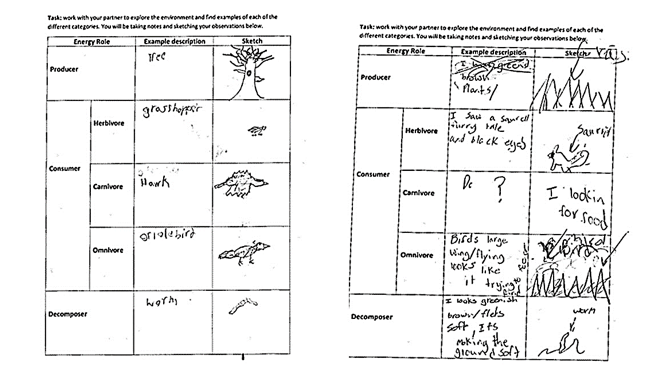
\includegraphics[width=\textwidth]{Figure 3e.png}
\end{figure*}

\clearpage
\subsection*{Explain}
The Explain, Elaborate, and Evaluate sections should collectively take one 60-minute class period. Following the outdoor exploration, students should return inside to complete the set of questions and draw their food web using the information they gathered outdoors. After students have completed this portion of the activity, they should discuss their recorded findings (Figure 3) with the whole class. Each group should share what they found and how the energy was transferred between their organisms within the food chain. At this point, the teacher should be sure to dispel any incorrect information or misconceptions regarding which organisms fall into which category. The teacher should also probe students for understanding by asking follow up questions such as: (a) Where did you see these organisms? (b) What habitat were they found in? (c) How do you know that this organism is a producer, consumer, decomposer? (d) What evidence can you provide for your categorization of these organisms? (e) What adaptations do the organisms have to survive in their habitat? In addition to discussing the scientific information, the teacher should also discuss the results of the partner protocol and checklist. Was it successful? What may have worked for the group or not worked and why? What will each pair do differently next time?

\begin{table*}[h!]
\captionsetup{font=large, labelfont=bf}
\caption{Exit Ticket Rubric}
\label{tab:Table-2}
\resizebox{\textwidth}{!}{%
\begin{tabular}{|l|l|l|l|}
\hline
\multicolumn{1}{|c|}{\textbf{Exceeding}} &
  \multicolumn{1}{c|}{\textbf{Meeting}} &
  \multicolumn{1}{c|}{\textbf{Approaching/Reteach}} &
  \multicolumn{1}{c|}{\textbf{Below/Intervene}} \\ \hline
\begin{tabular}[c]{@{}l@{}}Responses are accurate and \\ insightful.\\ Student connects more than \\ one key concept highlighted \\ in the question.\end{tabular} &
  \begin{tabular}[c]{@{}l@{}}Student connects more than \\ one key concept highlighted \\ in the question.\end{tabular} &
  \begin{tabular}[c]{@{}l@{}}Student responses partially address \\ the question.\\ Student provides 1 example to \\ support the response.\end{tabular} &
  \begin{tabular}[c]{@{}l@{}}Exit ticket is incomplete in \\ multiple sections or blank.\end{tabular} \\
\begin{tabular}[c]{@{}l@{}}Student provides 3 or more \\ examples to support the \\ response.\end{tabular} &
  \begin{tabular}[c]{@{}l@{}}Student Provides at least \\ 2 examples to support the \\ response.\end{tabular} &
  \begin{tabular}[c]{@{}l@{}}Student confuses or \\ misrepresents key concepts \\ while responding to questions.\end{tabular} &
  \begin{tabular}[c]{@{}l@{}}Student does not provide \\ any examples to support \\ the response.\end{tabular} \\ \hline
\end{tabular}%
}
\end{table*}

\subsection*{Elaborate}

The Explain, Elaborate, and Evaluate sections should collectively take one 60-minute class period. After students complete the discussion of outdoor observations, have the groups create information cards for each organism on their sheet. One side should include a picture of the organism and the other side should include information about habitat, what the organism consumes, and what consumes the organism. After these cards are completed, hand out the different organisms from the whole class randomly. Students wear these cards (either taped, or put in sheet protectors with string tied to each side) and stand in a circle. One student (randomly assigned) is given a ball of yarn. That student then passes the ball to another student who represents an organism who either consumes them or is consumed by them. Each time the yarn is passed, the student must provide a rationale for why they chose the specific organism. If students struggle to provide a rationale they can use the information on the back of the card for support. The yarn passing continues until all the organisms are holding onto the yarn. Have all students to take one step back and pull the string taut. Ask the students which of the organisms is the least important? Once they have identified the organism that they think is the least important, have that student drop their string. Then have all of the other organisms who feel a slack in the string drop their string. This should continue until all organisms have dropped their string. In this way, students should be able to see how things are all linked in an ecosystem and that all organisms are equally important. This web extends beyond just their simple drawings of a food chain and shows the interconnectedness between all organisms. The teacher should probe student understanding by asking: How are the needs of the different organisms met in our food chain? What would happen if an invasive species were introduced into this ecosystem? Why does the food web fall apart if one of the organisms is removed? How is matter flowing through this ecosystem?

\subsection*{Evaluate}

The Explain, Elaborate, and Evaluate sections should collectively take one 60-minute class period. In order to measure student knowledge and understanding of the lesson, which not only addressed the concept of producer, consumer, decomposer and energy transfer, but also focused on specific skills and practices based on collaboration and scientific argumentation, students will complete an exit ticket. Using an exit ticket and rubric (table 2) such as the one below, have students answer the questions before leaving the class for the day. Based upon the student rubric, scores of 1, 2, or 3, teachers can determine next steps for instruction.
 
 \subsubsection*{Exit Ticket}
 \begin{enumerate}
    \item List one producer, consumer and decomposer from the outdoor activity and describe how they are connected.
    \item Are all organisms important in the ecosystem investigated? Why or why not? Defend your answer using specific examples from class.
    \item If you are outside working in a partner team, what should you do if you and your partner cannot agree upon an idea to record? Why?
 \end{enumerate}

To provide the reader with an overview of the steps taken during this intervention and lesson, we offer a summary chart (Table 3). 

\clearpage
\begin{table}[h!]
\captionsetup{font=large, labelfont=bf}
\caption{Summary of Intervention Steps}
\label{tab:table-3}
\resizebox{\textwidth}{!}{%
\begin{tabular}{|l|l|l|}
\hline
\multicolumn{1}{|c|}{\multirow{2}{*}{\textbf{Lesson 1}}} &
  Engage: Matching Partners &
  \begin{tabular}[c]{@{}l@{}}Utilizing the Peer Assisted Learning Strategies approach,\\ the teacher will place students in groups.\end{tabular} \\ \cline{2-3} 
\multicolumn{1}{|c|}{} &
  \begin{tabular}[c]{@{}l@{}}Engage: Pre-Intervention\\ Activity\end{tabular} &
  \begin{tabular}[c]{@{}l@{}}Provide students with a collaborative task such as the one \\ suggested. During this task, the teacher should complete \\ the observation checklist (table 1) to identify student \\ behaviors throughout the class.\end{tabular} \\ \hline
\textbf{Lesson 2} &
  Explore: Intervention &
  \begin{tabular}[c]{@{}l@{}}1. Teacher facilitates the development of a collaboration \\ compliments list, providing positive language for students \\ to use during the activity (figure 1).\\ 2. Following the development of this list, the partner \\ protocol should be discussed to illustrate what a positive \\ learning experience should entail (figure 2).\\ 3. Students work in groups to complete the Exploration \\ Record Sheet based on prior knowledge and what they \\ think they will observe (figure 3) prior to going outside.\\ 4. Students go outside and complete the Exploration \\ Record Sheet (figure 3) based on actual observations.\end{tabular} \\ \hline
\multirow{3}{*}{\textbf{Lesson 3}} &
  Explain &
  \begin{tabular}[c]{@{}l@{}}Groups share what they found as they explored outdoors \\ and how the energy was transferred between their organisms \\ within the food chain. The teacher should facilitate this \\ discussion and use probing questions as needed to check \\ for understanding (figure 3).\end{tabular} \\ \cline{2-3} 
 &
  Elaborate &
  \begin{tabular}[c]{@{}l@{}}Students should create information cards for each organism \\ they observed outside. Using these cards, students illustrate \\ how all the organisms are interconnected within a food web.\end{tabular} \\ \cline{2-3} 
 &
  Evaluate &
  \begin{tabular}[c]{@{}l@{}}Students complete an exit ticket to check for understanding \\ of concepts taught during the three lessons. Teacher scores \\ this using rubric provided (table 2).\end{tabular} \\ \hline
\end{tabular}%
}
\end{table}
\clearpage
\section*{Outcomes}
As a result of this intervention, the teacher reported fewer behavioral challenges both in class, during instructional transitions, and in outdoor settings. Students appeared to benefit from the peer-based protocol and focus on positive verbal reinforcement throughout the activity. This outcome aligns with previous literature (Fox \& Avramidis, 2003), who found that opportunities in outdoor education significantly reduced challenges behaviors presented by children being educated in residential settings. Lane et al. (1983) also noted that students with Emotional and Behavioral Disabilities thrived socially when presented with opportunities to engage in outdoor education. Although multiple studies support our findings by highlighting the benefits of outdoor education, further investigations should be conducted to explore the impact of structured collaborative protocols. Given the positive outcomes cited in the current investigation, these studies will further add to the list of high leverage strategies that support children with and without disabilities during science-based educational opportunities.

\section*{Educational Importance}
Based upon the significant graduation and post-secondary concerns for students with Emotional and Behavior Disorders it is crucial for educators to address both academic and social-emoti\-onal needs (Data Resource Center for Child \& Adolescent Health, 2005/2006). The Peer Assisted Learning Strategies (PALS) approach combined with the 5e lesson is a way to enhance access and engagement for students with challenging behaviors. Literature suggests cooperative learning increases active student discussion, improves perceptions of social support, and strengthens friendships within the classroom setting (Kendrick et al., 2012). The connection to social support is critical given that theoretical frameworks cite social support as a buffer against stress and/or depression (Alloway \& Bebbington, 1987; Cassell, 1974; Cutro\-na \& Russell, 1990; Fiore et al., 1986; House, 1981; Lin \& Ensel, 1989). Therefore, the strong evidence surrounding peer-based intervention in the areas of academics and social-emotional wellness it is a promising tool to continue incorporating in inquiry driven science lessons (Fuchs, Fuchs, \& Burish 2000; Kendrick et al., 2012). 
 
There are many benefits to utilizing a structured collaborative learning format and peer-based protocols during outdoor science exploration. Specifically, peer-based interventions can potentially decrease challenging behaviors observed in class, during instructional transitions, and in outdoor settings. The intervention design supports the inclusion of students with Emotional and Behavior Disabilities using an observation tool, peer-based protocol, sentence stems for discourse guidance, hands-on activities, and ongoing opportunities for practice with specific feedback. Students should also benefit from the high levels of positive verbal reinforcement from classmates throughout activities to enhance social support. It is critical that we continue to strengthen collaborative opportunities among children experiencing social and academic challenges instead of simply denying access to less structured settings. This intervention provides a lens to replicate successful teaching and learning, using techniques and strategies that are most engaging for adolescents with varying needs enrolled in self-contained and inclusive classroom environments.

\include{} 
\section*{References}\par 

\leftskip 0.25in
\parindent -0.25in 
%%%
Alloway, R., \& Bebbington, P. (1987). The buffer theory of social support- a review of the 
literature. \textit{Psychological Medicine 17}, 91-108.

Anderman, E.M. (1998). The middle school experience: effects on the math and science 
achievement of adolescents with LD. \textit{Journal of Learning Disabilities. 31}, 128-138.

Bybee, R. (2014). The BSCS 5E Instructional Model: Personal Reflections and Contemporary
Implications. Science and Children.

Cassel J. (1974). An epidemiological perspective of psychological factors in disease etiology. 
\textit{American Journal of Public Health, 64}, 1040-1043.

Cutrona, C. E., \& Russell, D. W. (1990). Type of social support and specific stress: Toward a 
theory of optimal matching. In B. R. Sarason, I. G. Sarason, \& G. R. Pierce (Eds.), Wiley series on personality processes. Social support: An interactional view.

Data Resource Center for Child \& Adolescent Health. (2005/2006). National Survey of Children 
with Special Health Care Needs. Portland, OR: The Child and Adolescent Health Measurement Initiative (CAHMI). \url{childhealthdata.org/browse/survey/results?q=1099\&r=1}

Fiore, Coppel, Becker, \& Cox. (1986). Social support as a multifaceted concept: Examination of 
important dimensions for adjustment. \textit{American Journal of Community Psychology, 14}, 93-101.

Fox \& Avramidis (2003). An Evaluation of an Outdoor Education Programme for Students with 
Emotional and Behavioural Difficulties. \textit{Emotional and Behavioural Disabilities, 8}, 267-283.

Fuchs, D., Fuchs, L. S., \& Burish, P. (2000). Peer-assisted learning strategies: An evidence-
based practice to promote reading achievement.\textit{ Learning Disabilities Research and Practice}, 15(2), 85–91.

House, J.S. (1981). Work stress and social support. Reading, MA: Addison-Wesley.

Kendrick K, Jutengren G, Stattin H. (2012). The protective role of supportive friends against 
bullying perpetration and victimization.\textit{ Journal of Adolescence, 35}, 1069–1080.

Lane, B.J., Bonic, C. \& Wallgren-Bonic, N. (1983) ‘The Group Walk-Talk: A Therapeutic 
Challenge for Secondary Students with Social/Emotional Problems’, Teaching	 Exceptional Children16 (1): 12–17.

Sarason, I. G. \& G. R. Pierce (Eds.). \textit{Social support: An interactional view} (pp. 319-366). 
Oxford, England: John Wiley \& Sons.

Lin, N., \& Ensel W.M. (1989). Life stress and health: stressors and resources. \textit{American 
Sociological Review, 54}, 382-399.

Ryzin, M \& Roseth, C. (2019). Effects of cooperative learning on peer relationships, empathy, 
and bullying in middle school.\textit{ Aggressive Behavior, 45(6)}, 643-651.

U.S. Department of Education, Institute of Education Sciences, What Works Clearinghouse. 
(2012, June). Students with Learning Disabilities intervention report: Peer-Assisted Learning Strategies. Retrieved from \url{http://whatworks.ed.gov.}

\newpage

\section*{Connecting to the Next Generation Science Standards (NGSS Lead States 2013)}
\begin{itemize}
   \item The chart below makes one set of connections between the instruction outlined in this article and the \textit{NGSS}. Other valid connections are likely; however, space restrictions prevent us from listing all possibilities.
    \item The materials, lessons, and activities outlined in the article are just one step toward reaching the performance expectations listed below.
\end{itemize}

\clearpage
% Please add the following required packages to your document preamble:
% \usepackage{graphicx}
\begin{table}[]
\resizebox{\textwidth}{!}{%
\begin{tabular}{|ll|}
\hline
\multicolumn{2}{|l|}{\textbf{Standard 5-LS2 Ecosystems: Interactions, Energy, and Dynamics}} \\ \hline
\multicolumn{2}{|l|}{\textbf{\begin{tabular}[c]{@{}l@{}}Performance Expectation: 5-LS2-1. Develop a model to describe the movement of matter among \\ plants, animals, decomposers, and the environment.\end{tabular}}} \\ \hline
\multicolumn{1}{|l|}{\textbf{Dimension:}} &
  \textbf{Classroom Connection} \\ \hline
\multicolumn{1}{|l|}{\begin{tabular}[c]{@{}l@{}}\textbf{Science and Engineering Practice}\\ \href{https://nap.nationalacademies.org/read/13165/chapter/7#56}{Developing and Using Models}\end{tabular}} &
  \begin{tabular}[c]{@{}l@{}}Students create food chains to model what \\ they observed in the outdoor part of the lesson. \\ In addition, students participate in a food web \\ activity modeling the flow of energy from one \\ organism to another.\end{tabular} \\ \hline
\multicolumn{1}{|l|}{\begin{tabular}[c]{@{}l@{}}\textbf{Disciplinary Core Idea}\\ \textbf{LS2.A: Interdependent Relationships in Ecosystems}\\ The food of almost any kind of animal can be traced \\ back to plants. Organisms are related in food webs in \\ which some animals eat plants for food and other \\ animals eat the animals that eat plants. Some organisms, \\ such as fungi and bacteria, break down dead organisms \\ (both plants or plants parts and animals) and therefore \\ operate as “decomposers.” Decomposition eventually \\ restores (recycles) some materials back to the soil. \\ Organisms can survive only in environments in which \\ their particular needs are met. A healthy ecosystem is \\ one in which multiple species of different types are each \\ able to meet their needs in a relatively stable web of life. \\ Newly introduced species can damage the balance of an \\ ecosystem. (5-LS2-1)\end{tabular}} &
  \begin{tabular}[c]{@{}l@{}}Students investigate organisms within a habitat \\ and construct food chains and food webs to \\ illustrate the connections between the different \\ organisms and the transfer of energy. Students \\ make observations of different levels of \\ organisms in an ecosystem and construct a food \\ chain to illustrate understanding of the inter-\\ dependence of these individual organisms. \\ Additionally, students then utilize whole class \\ observations of organisms to construct a food \\ web expanding upon the flow of matter and \\ energy within the larger interconnected web or \\ organisms.\end{tabular} \\
\multicolumn{1}{|l|}{\begin{tabular}[c]{@{}l@{}}\textit{LS2.B}\\ \textit{\textbf{By the end of grade 5}}. Matter cycles between the air and\\ soil and among plants, animals, and microbes as these\\ organisms live and die. Organisms obtain gases, waters,\\ and minerals from the environment and release waster\\ matter (gas, liquid, or solid) back into the environment.\end{tabular}} &
  \begin{tabular}[c]{@{}l@{}}Students create food chains and food webs and \\ discuss how matter and energy flows throughout \\ each of them.\end{tabular} \\ \hline
\multicolumn{1}{|l|}{\begin{tabular}[c]{@{}l@{}}\textbf{Crosscutting Concept}\\ \href{https://nap.nationalacademies.org/read/13165/chapter/8#91}{Systems and System Models}\\ A system can be described in terms of its components \\ and their interactions. (5-LS2-1)\end{tabular}} &
  \begin{tabular}[c]{@{}l@{}}Students explore the different components of \\ their local ecosystem and discuss energy transfer \\ occurring between and among the organisms.\end{tabular} \\ \hline
\end{tabular}%
}
\end{table}

% Please add the following required packages to your document preamble:
% \usepackage{graphicx}
\begin{table}[]
\caption{Connections to the Common Core State Standards (NGAC and CCSSO 2010)}
\label{tab:table-4}
\resizebox{\textwidth}{!}{%
\begin{tabular}{|l|}
\hline
\textbf{ELA} \\
\begin{tabular}[c]{@{}l@{}}\href{http://www.corestandards.org/ELA-Literacy/SL/5/4/}{CCSS.ELA-Literacy.SL.5.4}\\ Report on a topic or text or present an opinion, sequencing ideas logically and using\\ appropriate facts and relevant, descriptive details to support main ideas or themes; \\ speak clearly at an understandable pace.\end{tabular} \\
\begin{tabular}[c]{@{}l@{}}\href{http://www.corestandards.org/ELA-Literacy/RI/5/7/}{CCSS.ELA-Literacy.RI.5.7}\\ Draw on information from multiple print or digital sources, demonstrating the ability \\ to locate an answer to a question quickly or to solve a problem efficiently.\end{tabular} \\ \hline
\end{tabular}%
}
\end{table}

\end{large}
\end{document}
